\documentclass[tikz, border=4pt]{standalone}
\usepackage{tikz}
\usepackage[all]{xy}
\begin{document}
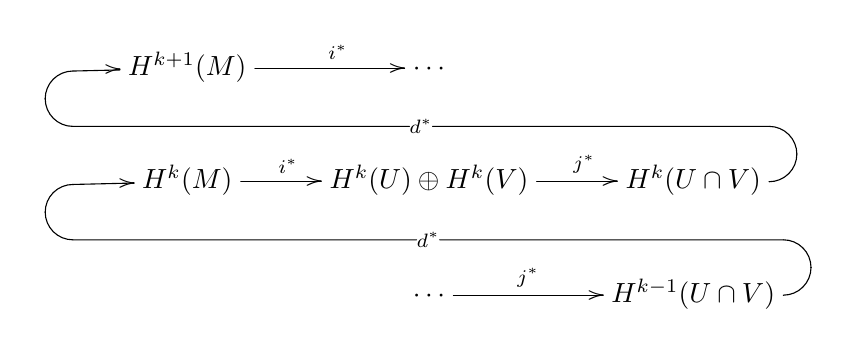
\begin{tikzpicture}[x=1cm, y=1cm]
  \node at (4.94,-1.77) {\pgfinterruptpicture%
  $\xymatrix{
  & H^{k+1}(M) \ar[r]^<<<<<<<<<<<{i^*} & \cdots \\
  & H^k(M) \ar[r]^>>>>>{i^*} 
  & H^k(U) \oplus H^k(V) \ar[r]^>>>>>{j^*} 
  & H^k(U \cap V) \ar `[ul] `[l] `[lllu] |{d^*} `[l] [rlllu] \\
  &  *{}  & \cdots \ar[r]^<<<<<<<<<<{j^*} 
  & H^{k-1}(U \cap V) \ar `[ul] `[l] `[lllu] |{d^*} `[l] [rlllu] }$%
  \endpgfinterruptpicture};
\end{tikzpicture}
\end{document}
